\begin{frame}{Projet 2 : Faucet React (front-end)}

  \begin{columns}
    \begin{column}{0.57\textwidth}
      Le but de ce projet est de créer une application web React qui aura pour but de permettre à un utilisateur de demander à recevoir des tokens ERC-20.
      Pour cette application, il faudra :

      \begin{itemize}
        \item créer un token ERC-20 de votre choix
        \item utiliser React (je suggère Next.js / Vite) et la bibliothèque Wagmi pour les smart contracts
        \item l'utilisateur appellera lui-même la fonction de mint
        \item bonus : inclure une limite de requêtes/montant par jour
      \end{itemize}
    \end{column}
    \begin{column}{0.37\textwidth}
      \resizebox{\textwidth}{!}{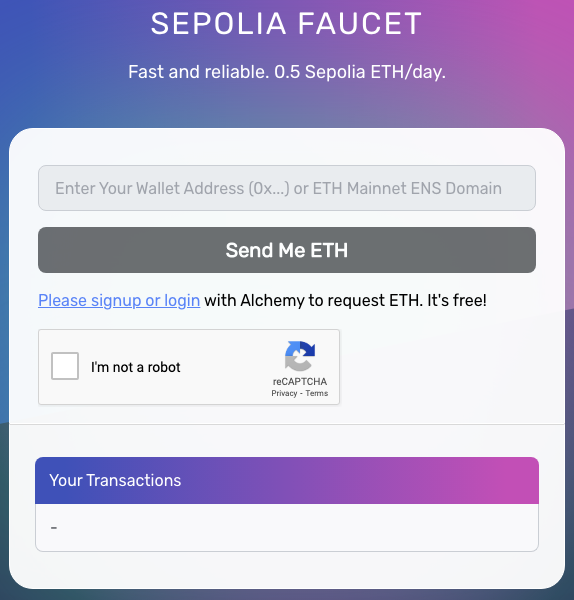
\includegraphics{img/faucet.png}}
    \end{column}
    \hspace{0.03\textwidth}
  \end{columns}
\end{frame}